In this section we will discuss the following:
\begin{enumerate}
    \item Results of the sensor data
    \item Results of the camera
    \item Results of the Lora module
\end{enumerate}
\section{Discussion of results of Sensor data}
in this section, the data gathered from the sensor will be discussed Note:(\textbf{all tests here were conducted indoors}):
\begin{enumerate}
    \item DHT22 (Temperature \& Humidity):

    On page \pageref{Recorded data from  DHT22 on the 5th of March} compared to the average room temperature which is  20$^o$c, The range of humidity in a room is from 30\% to 60\% in the plot on page \pageref{Temperature and Humidity plotted overtime} note in the file sensor\_data.csv there entries that are 0, this is due to testing different components and make these values as  0. during the development stage of this project we ran unit tests this module as seen on page \pageref{unit test message for DHT22 module}.
    \item AS312 (Motion ):

    As seen on page \pageref{Recorded data from AS312 on the \today} this will output a table that is True when an object is detected and  false when no object is  detected

    \item DFR0026 (Lux ):
    As seen on page \pageref{Recorded data from DFR0026 on the 25th of March 2024} is a table full of lux values according to this \href{https://www.thoughtco.com/lighting-levels-by-room-1206643}{link} we ideally want a lux value of  800 to 1700 lux which satisfies these conditions.
\end{enumerate}
\section{Discussion of Results of camera data}
As seen on page \pageref{A photo from 25th of March 2024} which shows  an image that was taken by the camera  attached to  the pi
\section{Discussion of Lora module}
\label{Discussion of Lora module}
While updating the repository for this section the Pi's SD cards were corrupted due to  a faulty binary file which was  later fixed  but  this error led to the following error message:

\begin{figure}[h!]
    \centering
    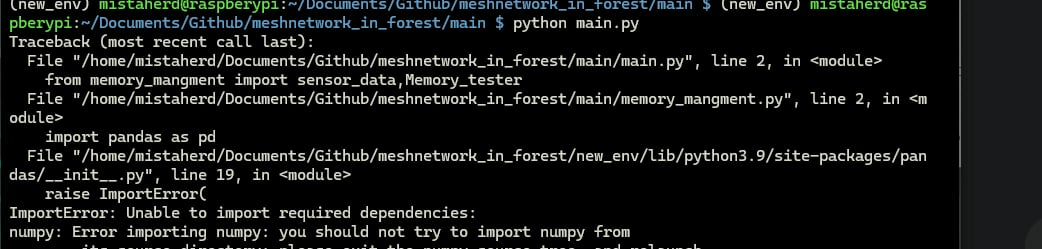
\includegraphics[width=0.5\linewidth]{Images/error_message.jpeg}
    \caption{environment error message}
    \label{environment error message}
\end{figure}